%{{{
\documentclass{beamer}
\usetheme{ensam}
\usepackage{pgfplots}
\usepackage{tcolorbox}
\usepackage{booktabs}
\usepackage{subcaption}
\usepackage{acronym}
\usepackage{tikz}
\usetikzlibrary{calc}
\usepackage{amsmath}
\usepackage {algorithmic}
\usepackage{algorithm}
\usepackage{eqparbox}
\usepackage[font=scriptsize]{caption}
\usetikzlibrary{bayesnet,positioning,calc}
\tikzstyle{obs} = [latent,fill=lightBlue]
\tikzstyle{default}=[draw=sexyRed,thick,rounded corners,text width=0.5in,font=\scriptsize,align=center]
\usepgfplotslibrary{colorbrewer}
%algorithmic comment
\renewcommand\algorithmiccomment[1]{%
  \hfill\comment{\#\scriptsize\eqparbox{COMMENT}{#1}}%
}
\renewcommand{\algorithmicrequire}{\textbf{Input:}}
\renewcommand{\algorithmicensure}{\textbf{Output:}}
\title{Variables Aleaoitres Discrete II}
\author{\underline{A.Belcaid}}
\institute{\small ENSA-Safi} 

%tikz bayesian theme
\usetikzlibrary{bayesnet,positioning,calc}
\tikzstyle{obs} = [latent,fill=lightBlue]
\tikzstyle{default}=[draw=sexyRed,thick,rounded corners,text width=0.5in,font=\scriptsize,align=center]
\DeclareMathOperator{\argmin}{argmin}

\pgfplotsset{every tick label/.append style={font=\tiny}}



% options for tcolorbox
\tcbset{fonttitle=\bfseries}
\acrodef{VA}{Variable Aleatoire}
\renewcommand{\P}{\mathbf{P}}
\newcommand{\E}{\mathbf{E}}
\newcommand{\var}{\text{var}}



\begin{document}
\maketitle
\begin{frame}
\tableofcontents
\end{frame}
\section{Variance}
\begin{frame}[<+->]
  \frametitle{Variance}
  \begin{itemize}
    \scriptsize
    \item Soit $X$ une \acf{VA} avec une esperance $\mu = \E[X]$.\\[4pt]
    \item On consiere alors la \ac{VA}  $X - \mu$.\\[4pt]
    \item Quelle sera l' \alert{\textbf{esperance}}  de $X - \mu$.\\[4pt]
  \end{itemize}
  \pause
  \begin{tcolorbox}[title=Variance]
   \small
   $$
   \var(X) = \E[\;\left(X - \mu\right)^2\;]
   $$
 \end{tcolorbox}

\begin{itemize}
  \scriptsize
  \item On peut la calculer en utilisant l'esperance d'une fonction d'une
    \ac{VA}.
    \small
    \begin{equation*}
      \var(X) = \sum_x \P_X(x) \left(x - \mu\right)^2
    \end{equation*}
  \item Une autre entite reliee a la \textbf{variance} est:
    \begin{tcolorbox}[title=Ecart type]
      $$
      \sigma(X) = \sqrt{\var\left(X\right)} $$
    \end{tcolorbox}
    
\end{itemize}
\end{frame}

\begin{frame}[t]
  \frametitle{Proprietes Variance}
  
  \begin{columns}
    \begin{column}{0.5\textwidth}
  \begin{itemize}
    \small
    \item<1-> On note $\mu = \E(X)$.\\[4pt]
    \item<2-> Soit $Y = X = b$, calculer 
          $$
          \var \left( Y \right) = 
          $$
          \vspace*{.5cm}
    \item<3-> On note $Y = aX$, calculer

          $$
          \var \left( Y \right) = 
          $$
  \end{itemize}
    \end{column}
    \begin{column}{0.5\textwidth}
      \only<4->
      {
        \begin{tcolorbox}
       $$
       \var(\left( aX + b\right) =  a^2 \var \left( X\right)
       $$
        \end{tcolorbox}
      }
    \end{column}
  \end{columns}
  \only<5->{
  On peut endeduire une formule utile pour le calcul de variance:
  
  \begin{tcolorbox}[title = Formule utile]
   $$
   \var(X) = \E[X^2] - \left(\E[X]^2\right)
   $$
  \end{tcolorbox}
}
\end{frame}

\begin{frame}[t]
  \frametitle{Variance d'une Bernoulli}
  on considere un \ac{VA}  qui suit une loi \alert{\textbf{Bernoulli}}.
  \begin{equation*}
    X = \begin{cases}
       1, & \text{\scriptsize avec prob } p\\ 
       0, & \text{\scriptsize avec prob } 1-p
    \end{cases}
  \end{equation*}
 \pause 
  \begin{itemize}
    \item Calculer la \alert{\textbf{Variance}}  de X avec formule normale:
      \begin{equation*}
        \var(X) = \sum_x ( x - \E[X])^2\P_X(x)
      \end{equation*}
  \end{itemize}
  \vspace*{1cm}
  \begin{itemize}
    \item Calculer la \alert{\textbf{Variance}}  de X en utilisant la deuxieme
      formule:
    
      \begin{equation*}
        \var(X) = \E(X^2) - (\E[X])^2
      \end{equation*}
  \end{itemize}
\end{frame}
\begin{frame}[<+->]
  \frametitle{Variance Loi Uniforme}
 \begin{columns}
   \begin{column}{0.5\textwidth}
     \scriptsize
    \only<2->{
      \begin{eqnarray*}
        \var[X] & =  & \E[X^2] - (\E[X])^2\\
                & = & \frac{1}{n+1} \left(\sum_{i=0}^n i^2\right) -
                \left(\frac{n}{2}\right)^2\\
                & = & \frac{n(n+1)(2n+1)}{6(n+1)} -  \left(\frac{n}{2}\right)^2\\[4pt]
                & = & \frac{n(n+2)}{12}
      \end{eqnarray*}
      
    }
    \only<3->{
      \scriptsize
      \begin{itemize}
        \item Pour le cas general entre $[a,b]$. on pose \alert{$n = b - a$}.
          \begin{equation*}
            \var(X) = \frac{1}{12}(b-a)(b-a + 2)
          \end{equation*}
      \end{itemize}
    }
   \end{column}
   \begin{column}{0.5\textwidth}
     \only<1->{
         \centering
         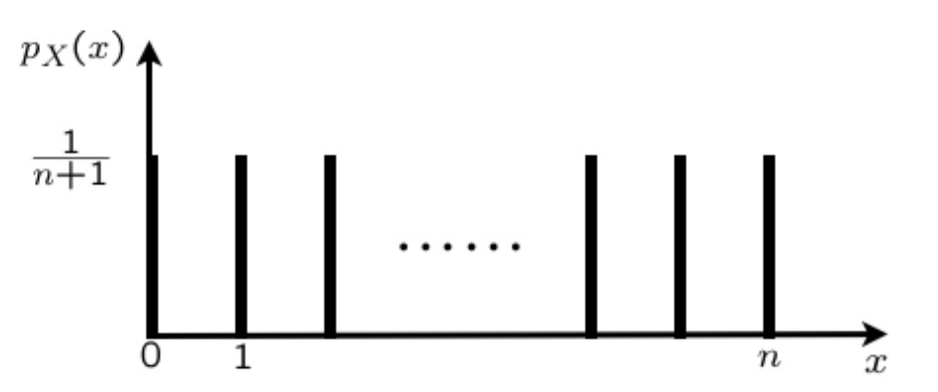
\includegraphics[width=0.8\textwidth]{./uniform_ref.png}
     }

     \vspace*{2cm}
     \only<3->{
         \centering
         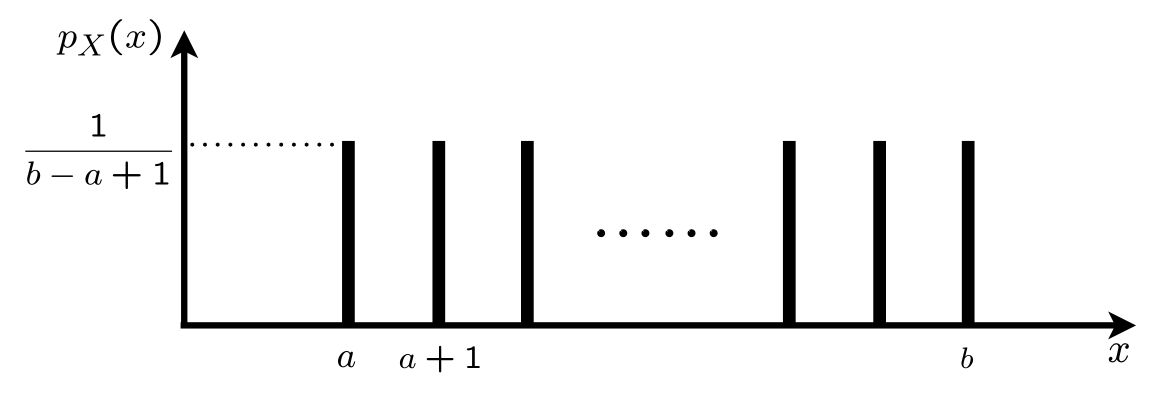
\includegraphics[width=0.8\textwidth]{./uniform_general.png}
     }
   \end{column}
 \end{columns} 
\end{frame}
\section{VA conditionnee sur une evenement}
\begin{frame}[t]
  \frametitle{Conditionement sur un evenement}
  \begin{itemize}
    \small
    \item On considere un evenement $A$ et on utilise la loi de \alert{probablite
      conditionnee sur $A$}.
  \end{itemize}
  \centering
  \scriptsize
  \vspace*{1cm}
  \begin{tabular}{m{5cm}m{5cm}}
   \toprule 
   \textbf{Loi Classique} & \textbf{Loi conditionnee}\\[8pt]
   \midrule
   $$ \P_X(x) = \P(X = x)$$ &  $$\P_{X|A}(x) = \P_X( X = x\;|\; A)$$ \\[3pt]
   $$ \sum_x\P_X(x) = 1$$ &  $$\sum_x\P_{X|A}(x) = 1$$ \\[3pt]
   $$ \E[X] = \sum_x x\cdot\P_X(x)  $$ &  $$\E[X|A] = \sum_x x\cdot\P_{X|A}(x)$$ \\[3pt]
   $$ \E[g(X)] = \sum_x g(x)\cdot\P_X(x)  $$ &  $$\E[g(X)|A] = \sum_x g(x)\cdot\P_{X|A}(x)$$ \\[4pt]
   \bottomrule
\end{tabular}
\end{frame}
\begin{frame}[t]
  \frametitle{Exemples}
 \begin{columns}
   \begin{column}{0.5\textwidth}
     \centering
     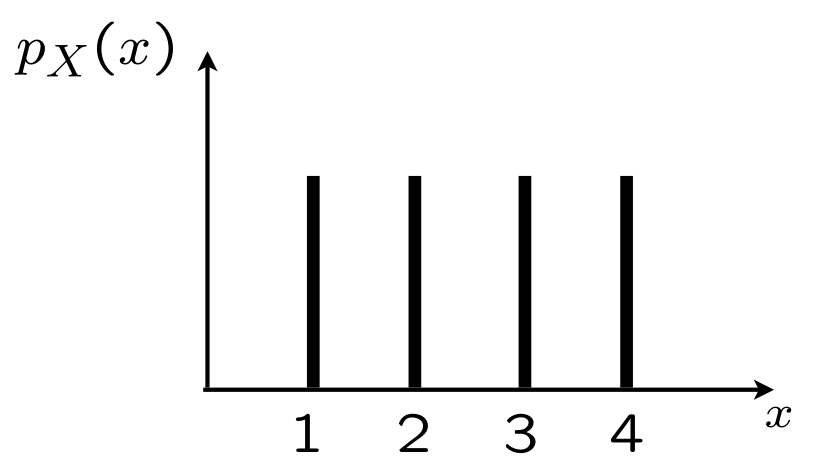
\includegraphics[width=0.8\textwidth]{./condition_example1.png}
     \vspace*{1cm}
        $$\E[X]=$$
        $$\var(X)=$$.
   \end{column}
   \begin{column}{0.5\textwidth}
    \only<2->{
      \begin{itemize}
        \small
      \item  On considere alors l'evenement \alert{$A={X \geq 2}$}
      \end{itemize}
      \vspace*{.5cm}
     \centering
     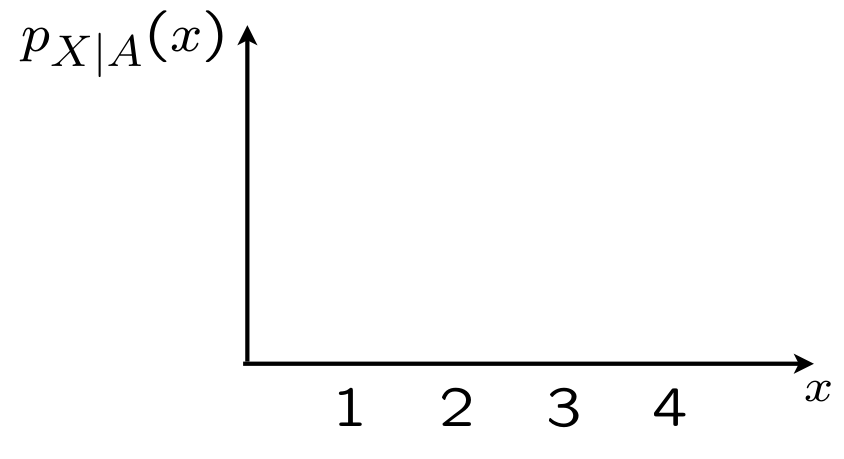
\includegraphics[width=0.8\textwidth]{./condition_example2.png}
     
     $$
     \E[X\;|\;A] = 
     $$

     $$
     \var(X\;|\;A) = 
     $$
    }
   \end{column}
 \end{columns} 
\end{frame}
\begin{frame}[t]
  \frametitle{Theoreme d'esperance totale}
 \begin{columns}
   \begin{column}{0.4\textwidth}
      \centering
      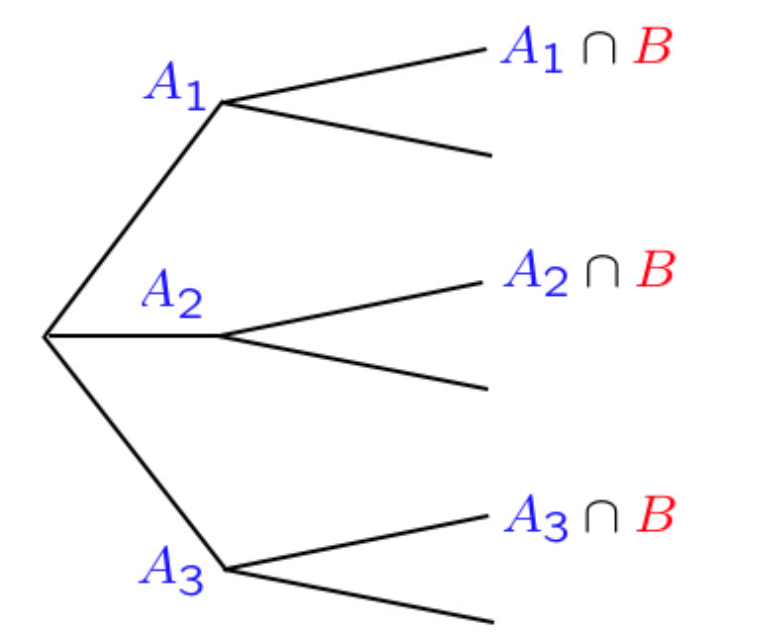
\includegraphics[width=0.8\textwidth]{./total_expectation.png}
      \pause
      
      \only<3->{
      \vspace*{2cm}
      \centering
      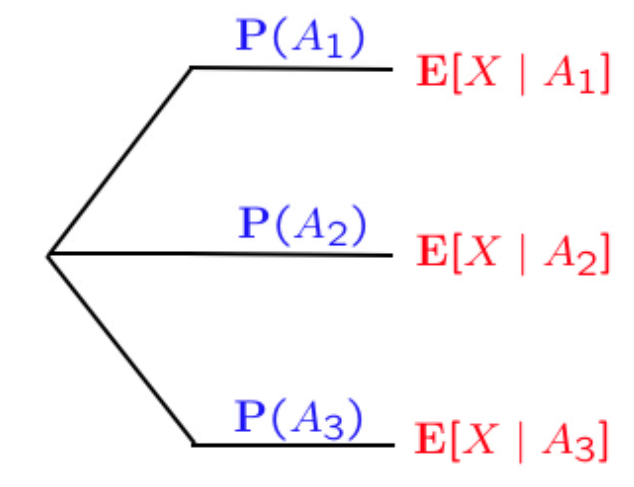
\includegraphics[width=0.8\textwidth]{./total_expectation2.png}
    }
   \end{column}
   \begin{column}{0.6\textwidth}
     \scriptsize
     \only<1->{
     $$
     P(B) = P_X(A_1)P_X(B|A_1) +  \ldots  + P_X(A_n)P_X(B|A_n)
   $$
 }
 \only<2->{
     $$
     P(x) = P_X(A_1)P_{X|A}(x) +  \ldots  + P_X(A_n)P_{X|A_n}(x)
     $$
   }
   \only<4->
   {
     \vspace*{1cm}
     \begin{tcolorbox}[title=Esparance totale]
       \scriptsize
      $$
      \E[X|A] = \sum_i^n \P(A_i)\E[X|A_i]
      $$
     \end{tcolorbox}
     
   }
   \end{column}
 \end{columns} 
\end{frame}
\begin{frame}[t]
  \frametitle{Exemple Esperance Totale}
 \begin{figure}[htpb]
   \centering
   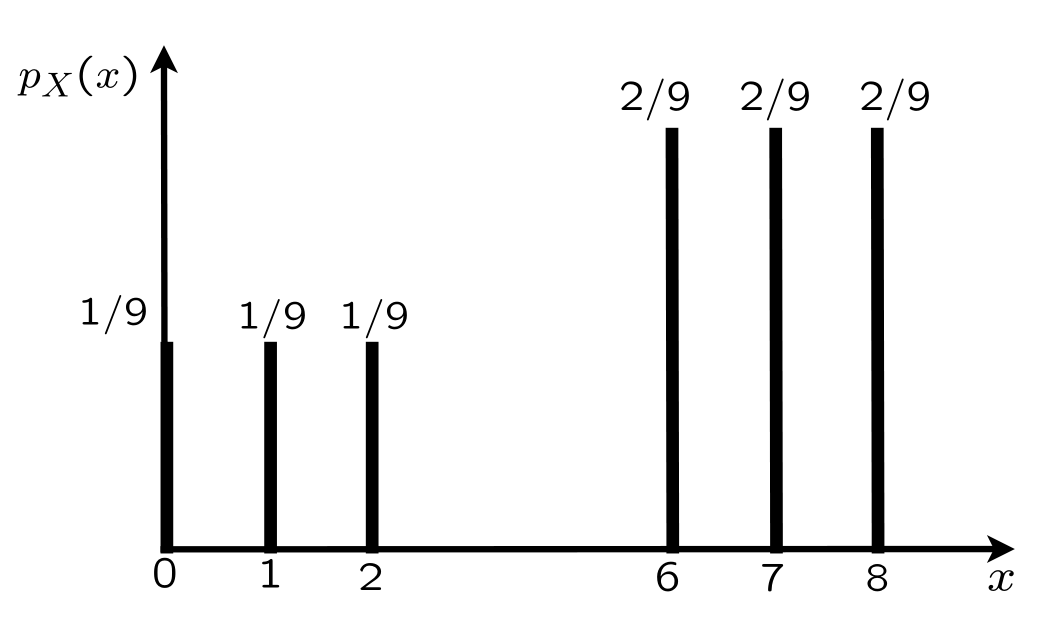
\includegraphics[width=0.7\textwidth]{./esperance_total_example.png}
   \caption{Calculer l'esperance de cette variable}
 \end{figure} 
 \pause
\end{frame}
\section{Multiples VAs}
\end{document}
